\subsection{Tests}

\paragraph{}
Pour tester notre algorithme nous avons eu besoin de deux choses :
\begin{itemize}
\item une fonction permettant de valider notre solution
\item un fonction permettant de générer aléatoirement des tests
\end{itemize}

\paragraph{}
La méthode \verb?isValid()? qui vérifie la validité de la solution calculée par notre algorithme est donnée par le pseudo-code suivant :
\begin{lstlisting}
isValid(ArrayList<Point> graph, ArrayList<Points> cds, int edgeTreshold) {
	valid = true;
	//build the graph structure of the cds
	ArrayList<NodeVertexDS> graphcds = graph(cds);
	
	//compute connex components
	for( v in graphcds ) {
		for( vn in v.neighbors ) {
			v.disjointsetelement.union(vn.disjointsetelement)
		}
	}
	
	compconnex = new HashSet<DisjointSetElement>();
	for( v in graphcds ) { compconnex.add(v.disjointsetelement.find()); }
	
	if(compconnex.size() > 1) { print("Error on connexity : " + compconnex.size()); valid = false) }
	
	rest = points.clone();
	rest.removeall(cds);
	
	//remove all neighbors of elements of cds from rest
	removeneighbors(rest, cds, edgeTreshold);
	
	if(rest.size() > 0) { print("Error dominating : " + rest.size()); valid = false; }
	
	return valid;
}
\end{lstlisting}

\paragraph{}
Nous avons aussi eu besoin de générer des tests. Pour cela il convient de générer des graphes géométriques de différentes tailles et avec des seuils différents (valeur maximale pour que 2 points soient considérés voisins l'un de l'autre).
Voici le pseudo code du générateur :
\begin{lstlisting}
generateGraph(width, heigth, nb, edgeTreshold) :
	result : ArrayList<Point>;
	while result.size() != nb :
		add random points in result until result.size() == nb
		compute connected components of result
		if there is multiple connected components :
			keep only the biggest connected components in points (remove the points that are in smaller components)
\end{lstlisting}

\paragraph{}
Nous avons ensuite établi plusieurs bases de test :

\begin{figure}[ht]
\begin{center}
\begin{tabular}{|*{3}{c|}}
    \hline
     Nombre de points  & Largeur $\times$ Hauteur  & Seuil \\
    \hline
    100  & 1000 $\times$ 1000 & 50 \\
    \hline
    500  & 1000 $\times$ 1000  & 50 \\
    \hline
    1000  & 1000 $\times$ 1000  & 50 \\
    \hline
    5000  & 1000 $\times$ 1000  & 50 \\
    \hline
    10000  & 1000 $\times$ 1000  & 50 \\
    \hline
\end{tabular}
\end{center}
\captionof{table}{Base de tests 1}
\end{figure}

\begin{figure}[ht]
\begin{center}
\begin{tabular}{|*{3}{c|}}
    \hline
     Nombre de points  & Largeur $\times$ Hauteur  & Seuil \\
    \hline
    100  & 1000 $\times$ 1000 & 5 \\
    \hline
    500  & 500 $\times$ 500  & 25 \\
    \hline
    1000  & 1000 $\times$ 1000  & 50 \\
    \hline
    5000  & 5000 $\times$ 5000  & 250 \\
    \hline
    10000  & 10000 $\times$ 10000  & 500 \\
    \hline
\end{tabular}
\end{center}
\captionof{table}{Base de tests 2}
\end{figure}

\begin{figure}[ht]
\begin{center}
\begin{tabular}{|*{3}{c|}}
    \hline
     Nombre de points  & Largeur $\times$ Hauteur  & Seuil \\
    \hline
    100  & 100 $\times$ 100 & 25 \\
    \hline
    500  & 500 $\times$ 500  & 36 \\
    \hline
    1000  & 1000 $\times$ 1000  & 50 \\
    \hline
    5000  & 5000 $\times$ 5000  & 161 \\
    \hline
    10000  & 10000 $\times$ 10000  & 300 \\
    \hline
\end{tabular}
\end{center}
\captionof{table}{Base de tests 3}
\end{figure}

Nous avons mené nos tests sur les 2 implémentations possibles du MIS dot les résultats ont été consignés sur les graphes suivants :

\begin{figure}
\begin{center}
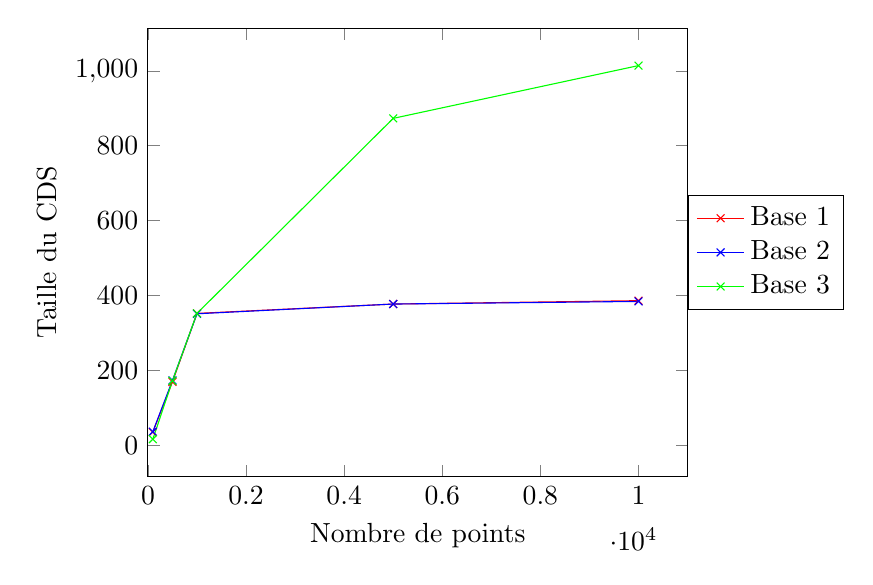
\begin{tikzpicture}
\begin{axis}[%
  xlabel=Nombre de points,
  ylabel=Taille du CDS,
  xmin=0,
  legend style={at={(1,0.5)},anchor=west},
]
  \addplot[color=red,mark=x]  coordinates {
	(100, 35)
	(500, 169)
	(1000, 352)
	(5000, 377)
	(10000, 386)
};
  \addlegendentry{Base 1}
  \addplot[color=blue,mark=x]  coordinates {
	(100, 36)
	(500, 173)
	(1000, 351)
	(5000, 377)
	(10000, 384)
};
  \addlegendentry{Base 2}
  \addplot[color=green,mark=x] coordinates {
  	(100, 16)
	(500, 172)
	(1000, 352)
	(5000, 873)
	(10000, 1014)
};
  \addlegendentry{Base 3}
\end{axis}
\end{tikzpicture}
\end{center}
\captionof{figure}{Taille du CDS en fonction du nombre de points avec MIS1}
\end{figure}

\begin{figure}
\begin{center}
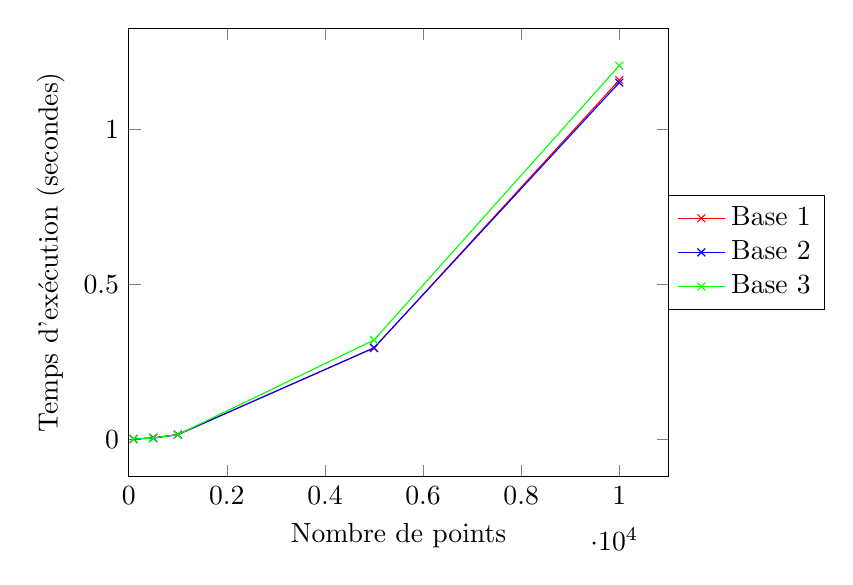
\begin{tikzpicture}[scale=1]
\begin{axis}[%
  xlabel=Nombre de points,
  ylabel=Temps d'exécution (secondes),
  xmin=0,
  legend style={at={(1,0.5)},anchor=west},
]
  \addplot[color=red,mark=x]  coordinates {
	(100, 0.00129)
	(500, 0.0046)
	(1000, 0.01495)
	(5000, 0.29473)
	(10000, 1.16013)
};
  \addlegendentry{Base 1}
  \addplot[color=blue,mark=x]  coordinates {
	(100, 2.0E-4)
	(500, 0.00398)
	(1000, 0.0149)
	(5000, 0.29543)
	(10000, 1.15217)
};
  \addlegendentry{Base 2}
  \addplot[color=green,mark=x] coordinates {
  	(100, 2.9E-4)
	(500, 0.0039)
	(1000, 0.01476)
	(5000, 0.32062)
	(10000, 1.20708)
};
  \addlegendentry{Base 3}
\end{axis}
\end{tikzpicture}
\end{center}
\captionof{figure}{Temps d'exécution en fonction du nombre de points avec MIS1}
\end{figure}

\begin{figure}
\begin{center}
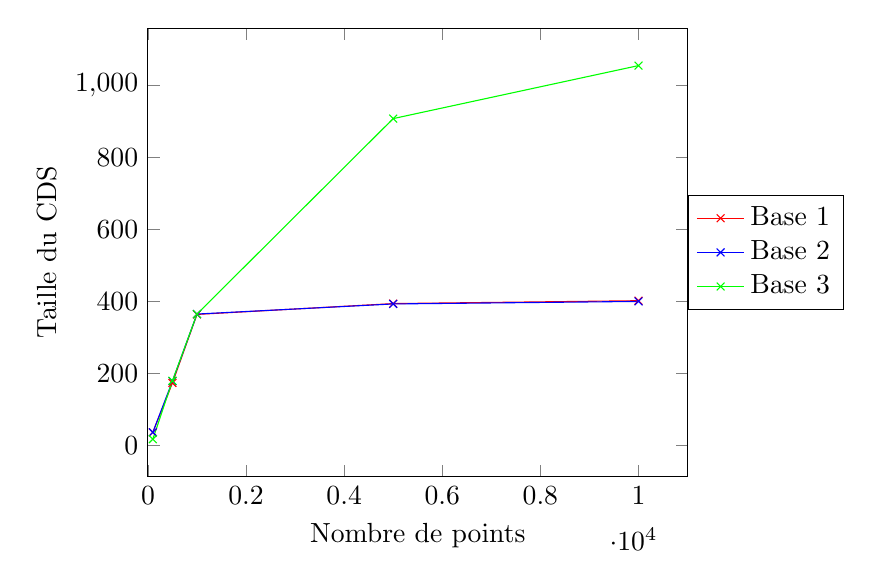
\begin{tikzpicture}
\begin{axis}[%
  xlabel=Nombre de points,
  ylabel=Taille du CDS,
  xmin=0,
  legend style={at={(1,0.5)},anchor=west},
]
  \addplot[color=red,mark=x]  coordinates {
	(100, 37)
	(500, 174)
	(1000, 364)
	(5000, 394)
	(10000, 402)
};
  \addlegendentry{Base 1}
  \addplot[color=blue,mark=x]  coordinates {
	(100, 37)
	(500, 179)
	(1000, 365)
	(5000, 393)
	(10000, 400)
};
  \addlegendentry{Base 2}
  \addplot[color=green,mark=x] coordinates {
  	(100, 18)
	(500, 180)
	(1000, 365)
	(5000, 907)
	(10000, 1054)
};
  \addlegendentry{Base 3}
\end{axis}
\end{tikzpicture}
\end{center}
\captionof{figure}{Taille du CDS en fonction du nombre de points avec MIS2}
\end{figure}

\begin{figure}
\begin{center}
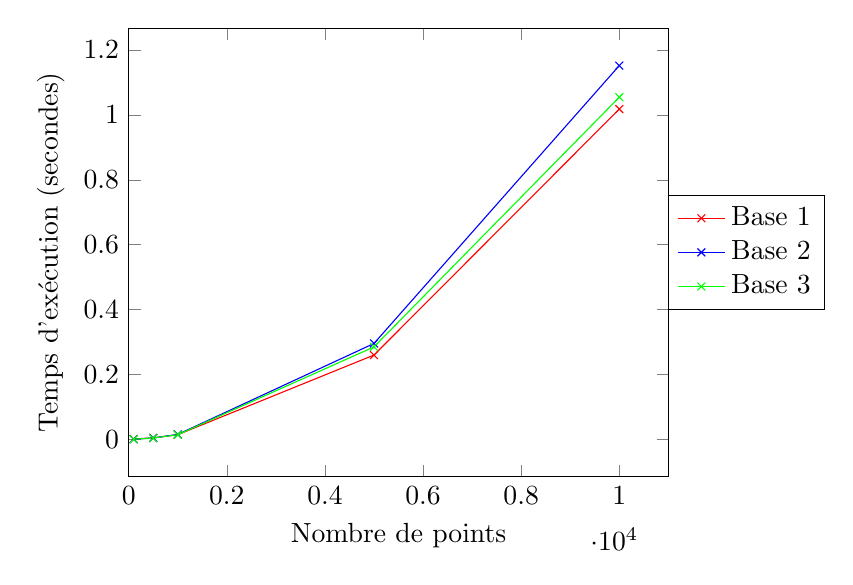
\begin{tikzpicture}
\begin{axis}[%
  xlabel=Nombre de points,
  ylabel=Temps d'exécution (secondes),
  xmin=0,
  legend style={at={(1,0.5)},anchor=west},
]
  \addplot[color=red,mark=x]  coordinates {
	(100, 9.1E-4)
	(500, 0.00425)
	(1000, 0.01403)
	(5000, 0.25969)
	(10000, 1.01815)
};
  \addlegendentry{Base 1}
  \addplot[color=blue,mark=x]  coordinates {
	(100, 2.4E-4)
	(500, 0.00398)
	(1000, 0.0149)
	(5000, 0.29543)
	(10000, 1.15217)
};
  \addlegendentry{Base 2}
  \addplot[color=green,mark=x] coordinates {
  	(100, 2.9E-4)
	(500, 0.00375)
	(1000, 0.01398)
	(5000, 0.28485)
	(10000, 1.0546)
};
  \addlegendentry{Base 3}
\end{axis}
\end{tikzpicture}
\end{center}
\captionof{figure}{Temps d'exécution en fonction du nombre de points avec MIS2}
\end{figure}